\documentclass{article}
\usepackage{amsmath, amssymb, mdwlist, graphicx, hyperref}


\newcommand{\mpar}[1]{\marginpar{\textit{#1}}}
\newcommand{\norm}[1]{\Vert #1 \Vert}
\DeclareMathOperator{\argmax}{argmax}
\DeclareMathOperator{\rank}{rank}
\DeclareMathOperator{\argmin}{argmin}
\newenvironment{solution}{\paragraph{Solution.}$\,$ }{\vskip 3mm\hrule}
\newenvironment{exercise}[2]{\begin{verse}\textbf{Exercise #1 (#2pt).} }{
\end{verse}\medskip}
\newcommand{\bbR}{\mathbb{R}}
\newcommand{\bw}{\mathbf{w}}
\newcommand{\bx}{\mathbf{x}}
\newcommand{\bd}{\mathbf{d}}
\newcommand{\bb}{\mathbf{b}}
\newcommand{\bs}{\mathbf{s}}
\newcommand{\bn}{\mathbf{n}}
\newcommand{\bF}{\mathbf{F}}
\newcommand{\ba}{\mathbf{a}}
\newcommand{\bc}{\mathbf{c}}
\newcommand{\bq}{\mathbf{q}}
\newcommand{\be}{\mathbf{e}}
\newcommand{\dd}{\mathrm{d}}
\newcommand{\pd}[2]{\frac{\partial #1}{\partial #2}}
\newcommand{\br}{\mathbf{r}}
\newcommand{\by}{\mathbf{y}}
\newcommand{\bzero}{\mathbf{0}}
\newcommand{\bz}{\mathbf{z}}
\newcommand{\bSigma}{\mathbf{\Sigma}}
\newcommand{\bp}{\mathbf{p}}
\newcommand{\bm}{\mathbf{m}}
\newcommand{\bM}{\mathbf{M}}
\newcommand{\bK}{\mathbf{K}}
\newcommand{\bD}{\mathbf{D}}
\newcommand{\bG}{\mathbf{G}}
\newcommand{\bA}{\mathbf{A}}
\newcommand{\bX}{\mathbf{X}}
\newcommand{\bY}{\mathbf{Y}}
\newcommand{\bP}{\mathbf{P}}
\newcommand{\bR}{\mathbf{R}}
\newcommand{\bI}{\mathbf{I}}
\newcommand{\bS}{\mathbf{S}}
\newcommand{\bT}{\mathbf{T}}
\newcommand{\balpha}{\boldsymbol{\alpha}}
\newcommand{\pt}[2]{\left(\begin{array}{c}#1\\#2\end{array}\right)}

\newcommand{\Bezier}{B\'{e}zier}

\newcommand{\vectwo}[2]{\left(\begin{matrix} #1 \\ #2 \end{matrix}\right)}

\begin{document}
\title{MTAT.03.015 Computer Graphics (Fall 2013)\\
\medskip
\Large Sample solutions to math exercises}
\author{Konstantin Tretyakov}
\date{}
\maketitle


\begin{enumerate}
\item Let $s$ be a straight line in $\bbR^2$, passing through the origin. It can be described parametrically as
$$
\bx = \lambda \bs, \qquad \lambda \in \bbR,
$$
or implicitly as
$$
\bn^T\bx = 0\,.
$$
Express the coordinates of the normal vector $\bn$ via the coordinates of the direction vector $\bs$.

\paragraph{Solution.} Fix a vector $\bs$ and consider a set of points $\{\bx:=\lambda \bs, \, \lambda \in \bbR\}$. The task is to find a vector $\bn$, such that for any $\lambda$ the condition
$$
\bn^T(\lambda \bs) = 0,
$$
is satisfied, and, vice-versa, if, for some $\bx$ it holds that $\bn^T\bx=0$ then it is necessarily true that $\bx = \lambda \bs$.

\emph{Necessity:} For simplicity, assume that\footnote{If it is not the case we can assume $s_2 \neq 0$ and proceed with the proof in the same way. If both $s_1 = s_2 = 0$ we must treat this as a special case and demonstrate that no matching $\bn$ exists then.}  $s_1 \neq 0$. Fix any $\lambda\neq 0$. Then,
\begin{align*}\
\bn^T(\lambda \bs) &= 0,\\
\bn^T\bs &=0,\\
n_1 s_1 + n_2s_2 &= 0,\\
n_1 &= -n_2s_2/s_1.
\end{align*}
Hence, if we pick any $t \in \bbR$ and construct $\bn$ as
$$
\bn = \left(\begin{array}{c} -ts_2/s_1 \\ t \end{array}\right)
$$
then all points of the form $\lambda \bs$ will also satisfy $\bn^T\bx = 0$.

Multiplying both sides by $s_1$ produces a somewhat more conventional answer:
$$
\bn = t\left(\begin{array}{c} -s_2 \\ s_1 \end{array}\right).
$$

\emph{Sufficiency:} We complete the proof by showing that for $t\neq 0$ any $\bx$ that satisfies $\bn^T\bx = 0$ (when $\bn$ is chosen as shown above) is also of the form $\bx = \lambda \bs$:

\begin{align*}
\bn^T\bx &= 0,\\
n_1 x_1 + n_2 x_2 &= 0,\\
-ts_2x_1 + ts_1 x_2 &= 0,\\
x_2 &= x_1s_2/s_1,\\
\bx &= \left(\begin{array}{c} x_1 \\ x_1s_2/s_1 \end{array}\right) = \left(\frac{x_1}{s_1}\right) \left(\begin{array}{c} s_1 \\ s_2\end{array}\right) = \lambda \bs.
\end{align*}

Consequently, for any direction vector $\bs$ the corresponding normal indeed exists and must be of the form 
$$
\bn = t\left(\begin{array}{c} -s_2 \\ s_1 \end{array}\right), \, t \neq 0.
$$
\item Let $\ba, \bb, \bc, \bd$ be points in $\bbR^2$. Find the coordinates of the intersection point of segments $[\ba, \bb]$ and $[\bc, \bd]$. Hint: Use the parametric representation.

\paragraph{Solution.}
The set of all points lying on the first segment can be parametrically described as
$$
\{\bx := t \ba + (1-t)\bb,\, t\in[0, 1]\}.
$$
Analogously, the set of point on the second segment is
$$
\{\bx := s \bc + (1-s)\bd,\, s\in[0, 1]\}.
$$
The intersection point must belong to both sets, and hence can be found by solving
$$
t \ba + (1-t)\bb = s \bc + (1-s)\bd.
$$
This is a system of two equations with two unknowns that can be solved using conventional means. Here is a more elegant solution by Raimond-Hendrik:
\begin{align*}
\bb + t(\ba - \bb) &= \bc + s(\bc-\bd),\\
\text{Box product on}&\text{ both sides with $(\bc - \bd)$,}\\
[(\bb + t(\ba - \bb))\times(\bc - \bd)] &= [(\bc + s(\bc-\bd))\times(\bc - \bd)],\\
\text{Linearity of the}&\text{ box product,}\\
[\bb\times(\bc - \bd)] + t[(\ba - \bb)\times (\bc - \bd)] &= [\bc\times(\bc - \bd)] + s[(\bc-\bd)\times(\bc - \bd)],\\
\text{Box product of }&\text{ a vector with itself is $0$,}\\
[\bb\times(\bc - \bd)] + t[(\ba - \bb)\times (\bc - \bd)] &= [\bc\times(\bc - \bd)],\\
t &= \frac{[\bc\times(\bc - \bd)] - [\bb\times(\bc - \bd)]}{[(\ba - \bb)\times (\bc - \bd)]}\\
t &=  \frac{[(\bc-\bb)\times(\bc - \bd)]}{[(\ba - \bb)\times (\bc - \bd)]}.
\end{align*}
Now if the denominator and the numerator are $0$, the segments lie on the same line. In this case we check whether the endpoints of one segment are within the other. If the denominator is $0$ and the numerator is not, the segments are parallel and do not intersect. If both are non-zero, it remains to check whether $t\in[0, 1]$ and if so, find the corresponding point as
$$t\ba + (1-t)\bb.$$

\item Prove that the (Euclidean) norm $\Vert \bx \Vert = \sqrt{\bx^T\bx}$ satisfies the \emph{triangle inequality}:
$$
\Vert \bx + \by \Vert \leq \Vert \bx \Vert + \Vert \by \Vert.
$$
Derive from this inequality also the inequalities 
$$\norm{\bx}-\norm{\by} \leq \norm{\bx - \by} \leq \norm{\bx} + \norm{\by}.$$

\paragraph{Solution.}
First part:
\begin{align*}
\Vert \bx + \by \Vert &\leq \Vert \bx \Vert + \Vert \by \Vert,\\
\Vert\bx + \by\Vert^2 &\leq \Vert\bx\Vert^2 + \Vert\by\Vert^2 + 2\Vert\bx\Vert\Vert\by\Vert,\\
(\bx + \by)^T(\bx+\by) &\leq \Vert\bx\Vert^2 + \Vert\by\Vert^2 + 2\Vert\bx\Vert\Vert\by\Vert,\\
\bx^T\bx + \by^T\bx + \bx^T\by + \by^T\by &\leq \Vert\bx\Vert^2 + \Vert\by\Vert^2 + 2\Vert\bx\Vert\Vert\by\Vert,\\
\bx^T\bx + 2\bx^T\by + \by^T\by &\leq \Vert\bx\Vert^2 + \Vert\by\Vert^2 + 2\Vert\bx\Vert\Vert\by\Vert,\\
\Vert\bx\Vert^2 + 2\bx^T\by + \Vert\by\Vert^2 &\leq \Vert\bx\Vert^2 + \Vert\by\Vert^2 + 2\Vert\bx\Vert\Vert\by\Vert,\\
\bx^T\by &\leq \Vert\bx\Vert\Vert\by\Vert.\\
\Vert\bx\Vert\Vert\by\Vert\cos\alpha &\leq \Vert\bx\Vert\Vert\by\Vert.\\
\end{align*}

Second part:
\begin{align*}
\Vert(\bx - \by) + \by\Vert  &\leq \Vert\bx - \by\Vert + \Vert \by \Vert \\
\Vert\bx\Vert  &\leq \Vert\bx - \by\Vert + \Vert \by \Vert \\
\Vert\bx\Vert - \Vert \by \Vert &\leq \Vert\bx - \by\Vert 
\end{align*}
and
\begin{align*}
\Vert\bx - \by\Vert = \Vert \bx + (-\by)\Vert  &\leq \Vert\bx\Vert + \Vert -\by \Vert = \Vert\bx\Vert + \Vert \by \Vert \\
\end{align*}

\item Let $\bp$ and $\bq$ be orthonormal vectors in $\bbR^3$. What transformation does the matrix $\bp\bp^T + \bq\bq^T$ correspond to? Prove it.

\paragraph{Solution.}
Intuitively, $\bp\bp^T$ is the orthogonal projector onto the axis defined by $\bp$. Similarly $\bq\bq^T$ is the projector onto the axis defined by $\bq$. Consequently, $\bp\bp^T+\bq\bq^T$ is an orthogonal projector onto the plane defined by $\bp$ and $\bq$.

Formally, let $\br$ be a third vector, that makes up an orthogonal basis together with $\bp$ and $\bq$. Pick any vector $\bx$. As $(\bp, \bq, \br)$ forms an orthonormal basis, we can represent $\bx$ in it, so let
$$
\bx = x_1\bp + x_2 \bq + x_3 \br.
$$
Now apply transformation $\bp\bp^T + \bq\bq^T$ to $\bx$:
\begin{multline*}
(\bp\bp^T + \bq\bq^T)(x_1\bp + x_2 \bq + x_3 \br) = \\x_1(\bp\bp^T + \bq\bq^T)\bp + x_2(\bp\bp^T + \bq\bq^T)\bq + x_3(\bp\bp^T + \bq\bq^T)\br = \\
x_1\bp + x_2\bq,
\end{multline*}
i.e. the transformation is indeed an orthogonal projector onto the $\bp$-$\bq$ plane.

\item Let $\bp$, $\bq$, $\br$ be an orthonormal basis in $\bbR^3$. Prove that $\bp\bp^T + \bq\bq^T + \br\br^T = \bI$, where $\bI$ denotes a unit matrix.

\paragraph{Solution.} Same as above. Show that for any $\bx = x_1\bp + x_2\bq + x_3 \br$ the application of $\bp\bp^T + \bq\bq^T + \br\br^T$ leaves the vector intact. This can only be the case when the transformation is the identity matrix. Alternative solution would be to note that
$$
\bp\bp^T + \bq\bq^T + \br\br^T
$$
is equal to $\mathbf{A}^T\mathbf{A}$, where $\mathbf{A}$ is the matrix with $\bp$, $\bq$, $\br$ as the rows. It easily follows then that $\mathbf{A}^T\mathbf{A} = \bI$.

\item Orthogonalize the following set of vectors using the Gram-Schmidt algorithm:
\begin{align*}
 \be_1 &= (\frac{\sqrt{2}}{2},\frac{\sqrt{2}}{2},0)^T \\
 \be_2 &= (-1, 1, -1)^T \\
 \be_3 &= (0, -2, -2)^T 
\end{align*}

\paragraph{Solution.}
Following the algorithm, pick the first vector as-is:
$$
 \be'_1 = \be_1 = (\frac{\sqrt{2}}{2},\frac{\sqrt{2}}{2},0)^T,
$$
Next, $\be'_2$ is $\be_2$ minus its projection onto $\be'_1$. As $\be'_1$ and $\be_2$ are already orthogonal, this projection is zero, hence in our case
$$
 \be'_2 = \be_2 = (-1, 1, -1)^T,
$$
Next, $\be'_3$ is $\be_3$ minus its projections onto $\be'_1$ and $\be'_2$. The vectors $\be'_2$ and $\be_3$ are already orthogonal, so we only need to subtract the projection onto $\be'_1$. Here we can further simplify by noting that $\Vert\be'_1\Vert$ = 1:
\begin{multline*}
 \be'_3 = \be_3 - \be'_1\be_1'^T\be_3 = (0, -2, -2)^T -  (\frac{\sqrt{2}}{2},\frac{\sqrt{2}}{2},0)^T \cdot (-\sqrt{2}) = \\
(0, -2, -2)^T + (1, 1, 0)^T = (1, -1, -2)^T
\end{multline*}

\item Compute the area of a triangle given by vertices
\begin{align*}
 \ba &= (1, 2, 3)^T, \\
 \bb &= (-2, 2, 4)^T, \\
 \bc &= (7, -8, 0)^T.
\end{align*}

\paragraph{Solution.}
Let $\bp = \bb - \ba$ and $\bq = \bc - \ba$. The area of the triangle is then simply half the length of the cross-product $\bp \times \bq$.
$$
S = \frac{1}{2}\Vert \bp \times \bq\Vert.
$$
Computing it with the given numbers:
\begin{align*}
\bp &= (-3, 0, 1)^T\\
\bq &= (6, -10, -3)^T\\
\bp\times \bq &= (10, -3, 30)^T\\
S &= \frac{1}{2} \sqrt{10^2 + 3^2 + 30^2} \approx 15.88
\end{align*}

\item Points $\bp_1, \bp_2, \dots, \bp_n \in \bbR^2$ are vertices of a simple polygon\footnote{A \emph{simple polygon} is a polygon, whose edges do not intersect each other.} listed in counter-clockwise order in a right-handed basis.
Prove that the area of the polygon $S$ can be computed as
\[
S = \frac{1}{2}(|\bp_1 \quad \bp_2| + |\bp_2 \quad \bp_3| + \dots + |\bp_n \quad \bp_1|)
\]
\paragraph{Solution.}
Recall that the expression $\frac{1}{2}|\bp\quad \bq|$ computes the signed area of the triangle $O\bp\bq$, where $O$ is the origin of the coordinate system. Now consider an example:
\begin{center}
\includegraphics[width=0.4\textwidth]{polygon1.png}
\end{center}
Note that the area ABCDEF can be computed as the difference between the area OABCDE = OAB+OBC+OCD+ODE, and the area OEFA = OEF + OFA. This is, however, exactly what the expression
$$
S = \frac{1}{2}(|A \quad B| + |B \quad C| + |C \quad D| + |D \quad E| + |E \quad F| + |F \quad A|)
$$
computes.
\begin{center}
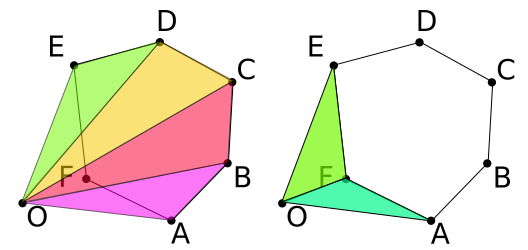
\includegraphics[width=0.8\textwidth]{polygon3.png}
\end{center}

The construction applies for any simple polygon.

\item Let $f: \bbR^m\to\bbR^n$ be a continuous function that satisfies $f(\bx + \by) = f(\bx) + f(\by)$ for each $\bx, \by$. Show that it then necessarily follows that for each $\alpha \in \bbR$ and each $\bx$
$$
f(\alpha\bx) = \alpha f(\bx),
$$\
i.e. $f$ must be linear.

\paragraph{Solution.}
\begin{enumerate}
\item First show that the required condition holds for any $\alpha = n \in \mathbb{N}^+$:
$$
f(n \bx) = f(\bx + \bx + \dots + \bx) = f(\bx) + f(\bx) + \dots + f(\bx) = nf(\bx).
$$
\item Now, for $\alpha = 0$:
$$
f(0) = f(0 + 0) = f(0) + f(0).
$$
which can only hold when $f(0) = 0$, i.e. $f(0\bx) = 0f(\bx)$.
\item For $\alpha = -1$:
$$
0 = f(\bx - \bx) = f(\bx) + f(-\bx), \text{ hence } f(-\bx) = -f(\bx).
$$
Consequently, condition holds for all $\alpha \in \mathbb{N}$.
\item Now let $\alpha = \frac{1}{m}$ for $m\in\mathbb{N}$.
$$
f(\bx) = f(m \frac{1}{m} \bx) = mf(\frac{1}{m}\bx),
$$
hence
$$
f(\frac{1}{m}\bx) = \frac{1}{m}f(\bx).
$$
\item Now, combining results (c) and (d), we conclude that condition holds for any rational $\alpha\in\mathbb{Q}$:
$$
f(\frac{n}{m}\bx) = nf(\frac{1}{m}\bx) = \frac{n}{m}f(\bx).
$$
\item Finally, let $\alpha \in \bbR$. Consider a sequence of rational numbers $\alpha_i$, that converges to $\alpha$:
$$
\lim_{i\to\infty} \alpha_i = \alpha
$$
Then, combining (e) and continuity of $f$:
\begin{align*}
f(\alpha \bx)&= f(\lim_i \alpha_i \bx) = \lim_i f(\alpha_i \bx) \\
             &= \lim_i \alpha_i f(\bx) = (\lim_i \alpha_i) f(\bx) = \alpha f(\bx).
\end{align*}
\end{enumerate}

\item
Consider a polyhedron with vertices $\bp_1, \bp_2, \dots, \bp_k$. Let $\bn_1$, $\bn_2, \dots, \bn_l$ be the normals for the faces of the polyhedron. Let us apply a linear transformation $\bF$ to all the vertices of the polyhedron. The vertices of the new polyhedron are thus $\bF\bp_1, \bF\bp_2, \dots, \bF\bp_k$. Express the normals of the new polyhedron in terms of the original normals.

\paragraph{Solution.}
Consider a face of the polyhedron, that includes vertices $\bp_1$ and $\bp_2$. The normal to this face $\bn_i$ must satisfy: $\bn_i^T(\bp_1-\bp_2) = 0$. Let $\bn'_i$ be the transformed normal. After transformation, the normal should stay perpendicular to the transformed face, i.e. it must hold that $\bn_i'^T(\bF\bp_1 - \bF\bp_2) = 0$.

Let $\bn_i' = (\bF^{-1})^T \bn$. Then
\begin{align*}
\bn_i'^T(\bF\bp_1 - \bF\bp_2) &= ((\bF^{-1})^T \bn)^T\bF(\bp_1 - \bp_2) \\
&= \bn^T\bF^{-1}\bF(\bp_1-\bp_2) \\
&= \bn^T(\bp_1-\bp_2) = 0.
\end{align*}

In fact it is easy to see that if we transform the normals using the matrix $(\bF^{-1})^T$ all the angles between normals and faces are preserved. The matrix $(\bF^{-1})^T$ is thus known as the \emph{normal transformation matrix}.



\item Let the horizontal field of view (\emph{fov-X}) of some \emph{view-frustum} be 75 degrees. Let the screen dimensions be $1280\times 1024$. Find the corresponding vertical field of view  (\emph{fov-Y}).

\paragraph{Solution.}
From
$$
\frac{\tan{(\text{fovX}/2)}}{\tan(\text{fovY}/2)} = \frac{1280}{1024}
$$
we compute
$$
\text{fovY} = 2\mathrm{arctan}\left(\frac{\tan(75/2)}{1280/1024}\right)\approx 63.09
$$

\item Consider a perspective projection in two-dimensional space. We shall be projecting to the line $y = 1$ with $(0, 0)$ as the center of projection.
\begin{itemize}
	\item Find the projection matrix in homogeneous coordinates.
	\item Explain what linear transformation does this matrix correspond to in the three-dimensional homogeneous space. Illustrations are welcome.
\end{itemize}
\paragraph{Solution.}
First, observe that the necessary transformation is
$$
(x, y)^T \to (x/y, 1)^T
$$
(see figure below). In homogeneous coordinates this would be
$$
(x, y, 1)^T \to (x/y, 1, 1)^T = (x, y, y)^T,
$$
which corresponds to the multiplication by the matrix
$$
\left(\begin{array}{ccc}1 & 0 & 0 \\ 0 & 1 & 0 \\ 0 & 1 & 0\end{array}\right)
$$
\begin{center}
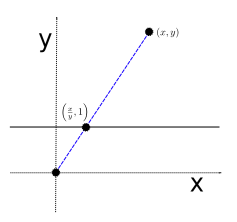
\includegraphics[width=0.5\textwidth]{projection1.png}
\end{center}

When viewed as a transformation $\bbR^3\to\bbR^3$, this matrix takes points from the $y=1$ plane and ``raises'' them up to $y=w$ plane. See illustration below. Think how perspective division after this transformation will lead all points back to the $w=1$ plane and, coincidentally, also the $y=1$ line.
\begin{center}
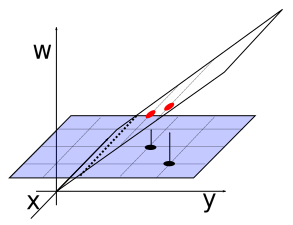
\includegraphics[width=0.5\textwidth]{projection2.png}
\end{center}

\item Let $ax + by + cz + d = 0$ be some plane in three-dimensional space and let $P = (p_x, p_y, p_z)$ be a point not located on this plane. Find a matrix, that performs a perspective projection from $P$ onto this plane (in homogeneous coordinates).
\paragraph{Solution.}
Let
\begin{align*}
\bw &:= (a,b,c,d),\\
k &:= (a^2 + b^2 + c^2)^{-1/2}\\
\bp &:= (p_x, p_y, p_z, 1),
\end{align*}
Now due to the properties of implicit plane equation, for any point $\bx = (x, y, z, 1)$ the signed distance from this point to the plane is equal to $k\bw^T\bx$. In particular, the distance from $P$ to the plane is $k\bw^T\bp$.

Now observe that the transformation we seek is the following:
\begin{center}
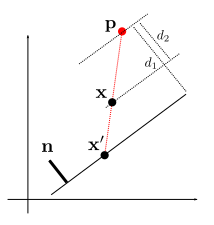
\includegraphics[width=0.5\textwidth]{projection3.png}
\end{center}
$$
\bx' = \bp + (\bx - \bp)\frac{d_1}{d_2} = \bp + (\bx - \bp)\frac{k\bw^T\bp}{k\bw^T\bp - k\bw^T\bx}
$$
Regrouping and simplifying:
\begin{align*}
(\bw^T\bp - \bw^T\bx)\bx' &= \bp(\bw^T\bp - \bw^T\bx) + (\bx - \bp)\bw^T\bp \\
&= \bp\bw^T\bp - \bp\bw^T\bx + \bx\bw^T\bp - \bp\bw^T\bp \\
&= (\bw^T\bp)\bx - \bp\bw^T\bx \\
&= ((\bw^T\bp)\bI - \bp\bw^T)\bx
\end{align*}
Recall that in homogeneous coordinates the points $\bx'$ and $\alpha\bx'$ are considered equivalent (for $\alpha \neq 0$), hence the left side of the above equation is already a representation of $\bx'$ (unless $(\bw^T\bp - \bw^T\bx) = 0$, i.e. the vector $\bp-\bx$ is perpendicular to the plane).

Consequently, the required transformation matrix in homogeneous coordinates is
$$(\bw^T\bp)\bI - \bp\bw^T.$$

It is straightforward to verify that the derivation holds for any $\bx$ independently of what side of the plane the point is located on (note that this affects the sign of $\bw^T\bx$).

\item Let $P_1 = (x_1, y_1, z_1)$, $P_2 = (x_2, y_2, z_2)$ -- be points in space. Consider some attribute $\mathcal{A}$ (e.g. color) assigned to the points. Suppose that point $P_1$ is assigned attribute value $a_1$, point $P_2$ --- value $a_2$ and on the line between them the attribute varies linearly.

Let $P_1^*$, $P_2^*$ --- be the perspective projections of points $P_1$ and $P_2$ onto the plane $z = z_n$ with $(0, 0, 0)$ as the center of projection.
Let $P_t^*$ be a point obtained by interpolating between $P_1^*$ and $P_2^*$: 
$$P_t^* = tP_1^* + (1-t)P_2^*,$$
and let $P_t = (x_t, y_t, z_t)$ be the point of the segment $[P_1, P_2]$ that projects into $P_t^*$. Show that the value $a_t$ of the attribute at point $P_t$ satisfies
\[ \frac{a_t}{z_t} = t \frac{a_1}{z_1} + (1-t)\frac{a_2}{z_2}\, .\]
Try to find a simple geometric proof to this fact.

It follows from this result, than when you are rasterizing a triangle, which was obtained via perspective projection, you cannot simply interpolate attribute values (e.g. colors or texture coordinates) along the screen as you did in the practice session\footnote{\url{http://en.wikipedia.org/wiki/Texture_mapping\#Perspective_correctness}}.

\paragraph{Solution.}
Intuitively, the following diagram explains the idea: depict $z$ on the horizontal axis and the attribute value on the vertical axis. The fact that screen coordinates vary linearly means that $\tan \alpha$ of the corresponding projection lines must vary linearly. The value of $\tan \alpha$ for each line is, however, exactly $a_i/z_i$.

\begin{center}
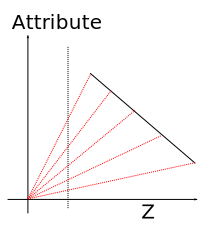
\includegraphics[width=0.5\textwidth]{interpolation1.png}
\end{center}

A more formal proof is given in Lengyel's book, Chapter 4.4.

%%%%%%%%%%%%%%%%%%%%%%%%%%%%%%%%%%%%%%%%%%%%%%%%%%%%%%%%%%%%%%%%%%%%%%%%%%%
\newpage

\item Bring examples of a two-piece linear spline curve, which happens to be:
\begin{enumerate}
\item $C^1$-smooth at the connection point.
\item $G^1$-smooth, but not $C^1$-smooth at the connection point.
\end{enumerate}

\paragraph{Solution.}
\begin{enumerate}
\item[(a)] Let the first piece be a segment between $(0, 0)$ and $(1, 0)$:
$$
\bp(t) = (1-t)\vectwo{0}{0} + t\vectwo{1}{0} = \vectwo{t}{0}
$$
and the second piece -- a segment between $(1, 0)$ and $(2, 0)$:
$$
\bq(t) = (1-t)\vectwo{1}{0} + t\vectwo{2}{0} = \vectwo{t+1}{0}
$$
The gradient of the first piece at the endpoint $\bp(1)$ is $(1,0)^T$, and is thus exactly equal to the gradient of the second piece at $\bq(0)$, hence the combined curve is $C^1$ (in fact, $C^\infty$)-smooth.

\item[(b)] Like in the previous case, let the first piece be a segment between $(0, 0)$ and $(1, 0)$:
$$
\bp(t) = (1-t)\vectwo{0}{0} + t\vectwo{1}{0} = \vectwo{t}{0}.
$$
Let the second piece be a segment, continuing from $(1,0)$ in the same direction, but faster, having $(3, 0)$ as the endpoint:
$$
\bq(t) = (1-t)\vectwo{1}{0} + t\vectwo{3}{0} = \vectwo{2t+1}{0}
$$
The gradient at $\bq(0)$ is $\bq'(0) = (2,0)^T = 2\cdot\bp'(1)$, i.e. the direction is the same, but the magnitude is different.
\end{enumerate}

\item Construct the basis matrices for:
\begin{enumerate}
\item the linear \Bezier' curve,
\item the quadratic \Bezier' curve.
\end{enumerate}

\paragraph{Solution.}
\begin{enumerate}
\item[(a)] By definition, the basis functions for a linear \Bezier' curve are
\begin{align*}
B^{(1)}_0(t) &= t^0(1-t)^{1-0} = (1-t), \\
B^{(1)}_1(t) &= t^1(1-t)^{1-1} = t,
\end{align*}
hence the basis matrix is
$$
\left(\begin{matrix} 1 & -1 \\ 0 & 1 \end{matrix}\right)
$$
\item[(b)] Analogously, the basis functions for a quadratic curve are
\begin{align*}
B^{(2)}_0(t) &= t^0(1-t)^{2-0}  = 1 -2t + t^2, \\
B^{(2)}_1(t) &= 2t^1(1-t)^{2-1} = 2t - 2t^2, \\
B^{(2)}_2(t) &= t^2(1-t)^{2-2} = t^2,
\end{align*}
hence the basis matrix is
$$
\left(\begin{matrix} 1 & -2 & 1\\ 0 & 2 & -2 \\ 0 & 0 & 1 \end{matrix}\right)
$$
\end{enumerate}

\item Construct the basis matrices for:
\begin{enumerate}
\item the linear Lagrange' curve,
\item the quadratic Lagrange' curve (assume the parameter vector for the control points to be $t=(0, 0.5, 1)$).
\end{enumerate}

\paragraph{Solution.}
\begin{enumerate}
\item[(a)] Following the construction of the Lagrange' basis matrix presented on the lecture, let
$$
\bA = \left(\begin{matrix} 0^0 & 1^0 \\ 0^1 & 1^1 \end{matrix}\right) = \left(\begin{matrix} 1 & 1 \\ 0 & 1 \end{matrix}\right)
$$
then the basis matrix is
$$
\bM_L = \bA^{-1} = \left(\begin{matrix} 1 & -1 \\ 0 & 1 \end{matrix}\right)
$$

\item[(b)] Analogously, let
$$
\bA = \left(\begin{matrix} 0^0 & 0.5^0 & 1^0 \\ 0^1 & 0.5^1 & 1^1 \\ 0^2 & 0.5^2 & 1^2 \end{matrix}\right) = \left(\begin{matrix} 1 & 1 & 1 \\ 0 & 0.5 & 1 \\ 0 & 0.25 & 1 \end{matrix}\right)
$$
hence the basis matrix is
$$
\bM_L = \bA^{-1} = \left(\begin{matrix} 1 & -3 & 2\\ 0 & 4 & -4 \\ 0 & -1 & 2 \end{matrix}\right)
$$
\end{enumerate}

\item Construct a one-dimensional quadratic Lagrange' curve defined by control points $(0, 1, 0)$. Provide the answer as a polynomial in $t$.

\paragraph{Solution.}
We seek for a parabola, that starts at $0$ for $t=0$, rises to $1$ at $t=0.5$ and then falls down to $0$ by time point $t=1$. Intuitively, it is easy to note that the polynomial must have $t=0$ and $t=1$ as its roots, hence it is of the form $\alpha t(t-1)$, where $\alpha$ can be found from the condition $\bp(0.5)=1$.
Alternatively, you might recognize the ``jumping'' motion path familiar to you from several practice sessions.

A more methodical way would be to follow the standard $\bP\bM\bT_2(t)$ formula together with the basis matrix derived in the previous exercise:
$$
\bp(t) = \left(\begin{matrix} 0 & 1 & 0 \end{matrix}\right)\left(\begin{matrix} 1 & -3 & 2\\ 0 & 4 & -4 \\ 0 & -1 & 2 \end{matrix}\right)\left(\begin{matrix} 1 \\ t \\ t^2 \end{matrix}\right) = 4t - 4t^2.
$$

\item Consider the curve in the previous exercise. Convert it to the \Bezier' representation. That is, find the \Bezier' control points for exactly the same curve.

\paragraph{Solution.}
Intuitively, it is possible to note that
$$
4t - 4t^2 = 2\cdot(2(1-t)t) = 0\cdot B^{(2)}_0(t) + 2\cdot B^{(2)}_1(t) + 0 \cdot B^{(2)}_2(t),
$$
hence the \Bezier' control points for the same polynomial must be $(0, 2, 0)$.

A more methodical approach is to follow the conversion method suggested on the lecture,
$$
\bP_B = \bP_L\bM_L\bM_B^{-1} = \left(\begin{matrix} 0 & 2 & 0 \end{matrix}\right)
$$

\item Prove that degree $n$ Bernstein polynomials $B_i^{(n)}, i\in\{0, \dots, n\}$ sum to one, i.e.:
$$
\sum_{i=0}^n B_i^{(n)}(t) = 1,\text{   for all   }n\in\mathbb{N}, t\in[0,1].
$$
Hint: one way to show it is to note that the Bernstein polynomials are somehow related to a well-known probability distribution.

\paragraph{Solution.}
If you are familiar with probability theory, you could note that $B^{(n)}_i(t) = \Pr[x=i]$ where $x$ is a random variable with a binomial distribution $\text{Bin}(n, t)$. Consequently,
$$
\sum_{i=0}^n B^{(n)}_i(t) = \sum_{i=0}^n \Pr[x=i] = \Pr[x\in\{0,\dots,n\}] = 1.
$$

More formally, we could use the binomial theorem:
$$
1 = 1^n = (t + (1-t))^n = \sum_{i=0}^n \vectwo{n}{i} t^i(1-t)^{n-i} = \sum_{i=0}^n B_i^{(n)}(t).
$$

\item A Hermite' curve is a reparameterization of the cubic \Bezier' curve, that is specified by its start and end points $\bp_0$, $\bp_3$ and its direction vectors (i.e. gradients) $\bs_0$, $\bs_3$ at those points. In other words, the geometry matrix for the Hermite' curve is $\bG=(\bp_0, \bp_3, \bs_0, \bs_3)$. Derive the basis matrix $\bM_H$ of the Hermite curve.

\paragraph{Solution.}
Recall that
\begin{align*}
\bs_0 &= 3(\bp_1-\bp_0)\\
\bs_3 &= 3(\bp_3-\bp_2)
\end{align*}
Consequently, the relationship between the Bezier' and the Hermite geometry matrices is:
\begin{align*}
\bP_H &= \left(\begin{matrix} \bp_0 & \bp_3 & \bs_0 & \bs_3\end{matrix}\right)
 = \left(\begin{matrix} \bp_0 & \bp_3 & (3\bp_1 - 3\bp_0) & (3\bp_3 - 3\bp_2)\end{matrix}\right) \\
&= \left(\begin{matrix} \bp_0 & \bp_1 & \bp_2 & \bp_3\end{matrix}\right) \left(\begin{matrix} 
1 & 0 & -3 & 0 \\ 
0 & 0 &  3 & 0 \\ 
0 & 0 &  0 & -3 \\
0 & 1 &  0 & 3
\end{matrix}\right) \\
&= \bP_B\bM
\end{align*}

Now, given a Bezier curve $\bp(t) = \bP_B\bM_B\bT_3(t)$, the equivalent Hermite representation would be
$$
\bp(t) = \bP_B\bM_B\bT_3(t) = (\bP_H\bM^{-1})\bM_B\bT_3(t)  = \bP_H(\bM^{-1}\bM_B)\bT_3(t),
$$
where the basis matrix is
$$
\bM^{-1}\bM_B = \left(\begin{matrix} 
1 & 0 & -3 & 2 \\ 
0 & 0 &  3 & -2 \\ 
0 & 1 &  -2 & 1 \\
0 & 0 &  -1 & 1
\end{matrix}\right)
$$

\item Prove that a cubic B-spline will pass a control point, if it is repeated three times.

\paragraph{Solution.}
Consider a segment of a cubic B-spline corresponding to four control points $\bp_0, \bp_0, \bp_0, \bp_3$ (i.e. the first point is repeated three times).
The corresponding curve segment (when represented via blending functions) is:
$$
\bp(t) = \bp_0 (b_0(t) + b_1(t) + b_2(t)) + \bp_3 b_3(t),
$$
However, $b_3(0) = \frac{0^3}{6} = 0$, hence $(b_0(0) + b_1(0) + b_2(0))$ must be $1$, and thus
$$
\bp(0) = \bp_0\cdot 1 + \bp_3\cdot 0 = \bp_0,
$$
i.e. the segment passes through $\bp_0$ at $t=0$.

Analogously, if the control points are $\bp_0, \bp_3, \bp_3, \bp_3$, then the curve is
$$
\bp(t) = \bp_0 b_0(t) + \bp_3(b_1(t) + b_2(t) + b_3(t)),
$$
and as $b_0(1) = \frac{(1-1)^3}{6} = 0$,
$$
\bp(1) = \bp_3,
$$
i.e. the curve passes through $\bp_3$ at $t=1$.

\item We derived the cubic B-spline to be a curve that is $C^2$-smooth at all points, no matter what the control points are. However, we also somewhy said that repeating control points ``reduces smoothness'' and even saw an example where repeating the control point three times results in a curve with a sharp corner. This seems like a contradiction. Explain this.

\paragraph{Solution.}
When a control point is repeated three times the curve will pass through it, which often results in visually sharp corners. Surprisingly, however, the curve function will still stay $C^2$-smooth. This happens because, in terms of movement, the curve ``comes to a halt'' at the repeated control point (its first and second derivatives become zero for a moment), and then gradually builds up speed in a different direction.

To see it better, consider a one-dimensional B-spline with control points $0.5, 3, 3, 3, 1$ as a function of $t$:
\begin{center}
\includegraphics[width=0.7\textwidth]{bspline1d.png}
\end{center}

Note how the curve moves in a positive direction, reaches the point $3$ at $t=2$, halts there for a moment and starts moving backwards away from $3$. If you visualize this movement as a one-dimensional curve viewed ``from above'', you might mistake this for a $C^2$-discontinuity.

Note that this makes the effect of repeating control points different from the effect of repeating knots in a non-uniform B-spline. In the latter case the basis functions really loose smoothness. See image below.

\begin{figure}[h]
\centering
\includegraphics[width=0.7\textwidth]{nurbs.png}
\begin{minipage}{0.9\textwidth}
The basis functions of a four-control-point 3$^\text{rd}$ degree NURBS curve with knot vector $(0,1,2,2,2,3,4,5)$. Note how the second basis function is not $C^1$-smooth at $t=2$, and hence the whole curve will not be.
\end{minipage}
\end{figure}

\item Prove that a (uniform) B-spline of degree $k$ with $n$ control points has $n+k+1$ knots. 

Hint: count the number of curve segments and add the ``virtual'' segments on both sides, where the basis functions for the first and last control points are still nonzero.

\paragraph{Solution.}
A single segment of a degree $k$ B-spline, being a polynomial curve, is determined by $k+1$ control points. Consequently, one control point affects $k+1$ different segments of the spline, i.e. it is weighed by a basis function that must span $k+2$ knots (the parameter values, corresponding to endpoints and connection points of $k+1$ segments). This proves that for $n=1$ the total number of knots is indeed $n+k+1$.

Now add a new control point. This introduces a new basis function. The domain of the added basis function includes $k$ previous segments and 1 new (see illustration below). Consequently, one extra knot needs to be added for each new control point. For $2$ points there will thus be $2+k+1$ knots, for $3$ points $3+k+1$ knots, and the claim holds by induction.

Alternatively, note that the parameter region where the basis function of the control point $\bp_i$ is nonzero is $[i, i+k+2]$. Consequently, the parameter space where at least one basis function is nonzero starts at $0$ (the leftmost end of the basis function for $\bp_0$) and ends at $(n-1)+k+2$ (the rightmost end of the basis function for $\bp_{n-1}$).

\begin{figure}[h]
\centering
\includegraphics[width=0.7\textwidth]{knotcount.png}
\begin{minipage}{0.9\textwidth}
Two consecutive basis functions of a 4th degree B-spline. Each spans $5$ segments and thus requires $6$ knots. The two functions share a region of $4$ common segments. The total number of knots is $7=4+2+1$.
\end{minipage}
\end{figure}
\end{enumerate}
\end{document}

